\documentclass[12pt,a4paper]{article}
\usepackage[utf8]{inputenc}
\usepackage[french, activeacute]{babel}
\usepackage{amssymb}
\usepackage{amsmath}
\usepackage{graphicx}
\usepackage{wrapfig}
\usepackage{eurosym}
\usepackage{url}
\usepackage{mathpazo}
\usepackage[T1]{fontenc}
\usepackage[inner=3cm, outer=3cm, bottom=2.5cm, top=2cm]{geometry}

\hyphenation{ré-ac-tions}
\hyphenation{ré-ac-tion}
\hyphenation{no-yaux}

\date{17 janvier 2010}

\title{Les centrales nucléaires à fusion: Une source d'électricité propre, durable et sécuritaire?}

\author{Matthias Reis}


% TODO: cela / celui, la quelle / le quel ??

\begin{document}
\maketitle \newpage
\tableofcontents \newpage

\section{Introduction}
La fusion nucléaire est une réaction où deux noyaux atomiques s'assemblent pour former un noyau plus lourd. Elle est donc un processus qui fait pendant à la fission nucléaire où le noyau d'un atome lourd est divisé en plusieurs nucléides plus légers. Aujourd'hui, il y a deux principales motifs pour l'étudier: %TODO: Militaerische Motivation!!!

D'abord, il y a une fascination pour ce processus élémentaire de la nature qui prend place dans le noyau de presque toutes les étoiles. Sans la fusion nucléaire, le soleil n'émettrait pas d'énergie et la vie sur la terre ne serait pas possible.

Deuxièmement, on espère à utiliser les grandes quantités d'énergie libérées pendant la réaction pour l'alimentation en énergie. On promet une source d'énergie qui n'émettrait pas de gaz à effet de serre, ne produirait pas de déchets nucléaires d'une durée de vie longue et disposerait des carburants presque inexhaustibles. En outre, une centrale à fusion nucléaire serait <<intrinsèquement>> sécuritaire car une réaction en chaîne incontrôlée ne serait pas possible à cause des quantités petites de carburant qui seraient présentes dans le réacteur\footnote{HiPER Technical background and conceptual design report \cite{hiper}, p. 13}.

En suivante, je vais d'abord introduire les principes fondamentales de la fusion avec leur réalisations techniques et présenter les possibles impacts sur la société et l'environnement en dernière partie. 

\section{Les principes fondamentales de la fusion}
%\subsection{Les réactions nucléaires relevantes}
Quand deux noyaux atomiques s'assemblent pour former un noyau nouveau, la somme des masses des noyaux antérieurs est plus grand que la masse du noyau nouveau, un effet qu'on appelle \textit{défaut de masse}. La différence entre la masse des noyaux antérieurs et du noyau nouveau est convertie en énergie.

\begin{figure}[htb]
	\centering 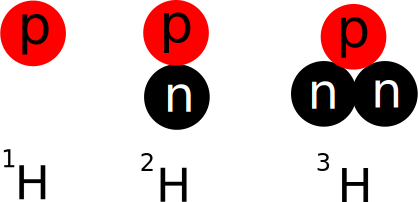
\includegraphics[width=0.5\textwidth]{images/IsotopesH}
	\caption{Les isotopes de l'hydrogène: L'hydrogène (\textsuperscript{1}H), le deutérium (\textsuperscript{2}H) et le tritium (\textsuperscript{3}H). Les cercles noirs correspondent aux neutrons (des charges neutres), les cercles rouges référent aux protons (des charges positives).}
	\label{fig:deutrit}
\end{figure}
La fusion plus facile à réaliser en terre est la réaction entre deutérium et tritium (fig. \ref{fig:deutrit} et \ref{fig:deutritFusion}), deux isotopes naturels de l'hydrogène:
\begin{equation}
^2 \text{D} + ^3 \text{T} \rightarrow ^4\text{He} ~( 3,5 ~\text{MeV} ) + \text{n}^0 ~( 14,1 ~\text{MeV} ) \label{eqn:DTfusion}
\end{equation}
Le produit de cette réaction est un noyau de hélium avec l'énergie de $3,5$ MeV (megaélectron-volt, une unité de mesure d'énergie) et un neutron avec l'énergie de $14,1$ MeV. Dans les réacteurs à fusion, on utilise ce neutron pour deux buts:
\begin{enumerate}
\item La production d'éléctricité: D'abord, le rayon de neutrons est absorbé par un confinement qui se chauffe en conséquence. Pour convertir cette chaleur en électricité, on emploie une installation thermique qui produit de la vapeur transformée en énergie mécanique et puis en énergie électrique au moyen d'une turbine à vapeur, comme dans les centrales conventionnelles. 
\item La production de tritium dont la réaction a besoin (voir \ref{dt}).
\end{enumerate}

\begin{figure}[htb]
	\centering 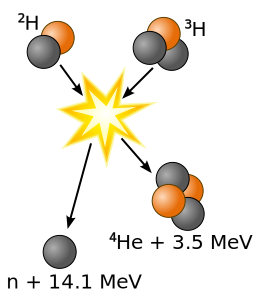
\includegraphics[width=0.5\textwidth]{images/Deuterium-tritium_fusion}
	\caption{La fusion de deuterium et tritium. Source: \cite{fusionwiki}}
	\label{fig:deutritFusion}
\end{figure}
Il existe naturellement une répulsion entre deux noyaux car les deux ont une charge électriquement positive. Pour faire la fusion de deux noyaux possible, il faut que les noyaux puissent surmonter la \textit{barrière coulombienne} due à leurs charges électriques. C'est pour ça que la fusion nucléaire normalement ne prend place que dans le noyau des étoiles, où la masse énorme de l'étoile crée une pression qui est assez puissante à approcher les noyaux suffisamment. La conséquence est donc qu'il faut d'abord investir d'énergie pour que la réaction soit possible et les noyaux puissent surmonter la barrière coulombienne. Pour ça, il est nécessaire de construire quelque mécanisme pour créer les conditions propres d'une réaction de fusion.

%Le but de beaucoup des expériences grandes n'est pas exclusivement fusionner des noyaux mais plutôt lancer une réaction qui se entretient à soi-même. Pour ça, il est nécessaire de lancer de l'extérieur tant de processus à fusion que l'énergie des noyaux d'hélium dans la réaction (eq. \ref{eqn:DTfusion}) suffisse pour fusionner les noyaux de deutérium et tritium de nouveau. Dans le cas de succès, ce processus est appelé <<l'allumage>> car on a allumé <<le feu nucléaire>>. On n'a jamais réalisé ce but d'une manière contrôlée, en fait les explosions des bombes H étaient les seules fois où une telle réaction a été réalisé par l’homme. Il faut dire quand même qu'une telle réaction n'est pas nécessaire pour produire d'électricité blablabla... dieser abschnitt ist bullshit

\section{Les possibles réalisations techniques}
Pour gagner d'énergie, une installation qui peut lancer la réaction de fusion ne suffit pas, quelque chose qui est réalisé depuis les années 1950 dans l'Union Soviétique. Il faut plutôt construire un réacteur qui consomme moins d'énergie pour maintenir les réactions nucléaires que la fusion produit. Les deux réalisations techniques plus courantes qui pourraient remplir les exigences sont présentées en suivante.
%TODO: Ökonomisch: Entwicklungskosten, Wartungskosten, Betriebskosten?

\subsection{La fusion par confinement inertiel}
Le confinement inertiel fonctionne à base de l'inertie des combustibles. Dans cette voie, l'énergie est apportée par un faisceau de lumière laser ou bien par un faisceau de particules chargées (électrons ou ions) à une bille de combustible de quelques millimètres de diamètre. Comme l'énergie est apportée à une quantité énorme pendant une période de temps très courte, les combustibles ne peuvent pas enfuir grâce à leur inertie. Comme ça, la concentration de particules exigée et donc l'allumage peut être réalisée. Ensuite la réaction nucléaire s'éteint à cause du refroidissement du combustible pendant quelques $10^{-8}$ - $10^{-7}$ secondes. Les lasers qui sont installées dans la <<National Ignition Facility>> (NIF) à Livermore (Californie, États-Unis), l'expérience plus grande de fusion par confinement inertiel (budget : 4,2 milliards de dollars), peuvent répéter ce processus jusqu'à 4 - 6 fois par jour. Pour produire d'électricité à cette façon, on a besoin d'une fréquence de 10 - 15 impulsions de laser par seconde\footnote{\url{https://lasers.llnl.gov/about/missions/energy_for_the_future/life/benefits_challenges.php}}.

Un concept nouveau qui s'appelle <<Fast Ignition>> (en français: <<allumage ra\-pide>>) et promet d'atteindre des gains d'énergie beaucoup plus hauts est projeté sous le nom <<HiPER>> (<<High Power Laser Energy Research>>, en français : <<Projet Laser haute puissance>>). Pour l'expliquer, on emploie une analogie avec le moteur à combustion. Dans cette modèle, la méthode d'allumage de la NIF fait pendant à un diesel car le combustible est comprimé et puis s'allume. Le pendant du moteur à essence serait exactement le principe de l'allumage ra\-pide: D'abord, le combustible est comprimé avec un faisceau de laser moins puissant que celui de la NIF. Ce faisceau fait donc pendant au piston dans le moteur. Quand le combustible est assez comprimé et donc assez chaud, un second faisceau de laser plus puissant produit un rayon d'électrons dans le combustible (le pendant de l'étincelle d'allumage) qui lance finalement les réactions nucléaires (fig. \ref{fig:FastStages}). Comme c'était un problème dans beaucoup des expériences de réaliser la compression autour du combustible assez symétrique et puissant, le concept de l'allumage ra\-pide promet un avantage grand à cause des exigences moindres au faisceau du laser comprimant.
\begin{figure}[htb]
	\centering 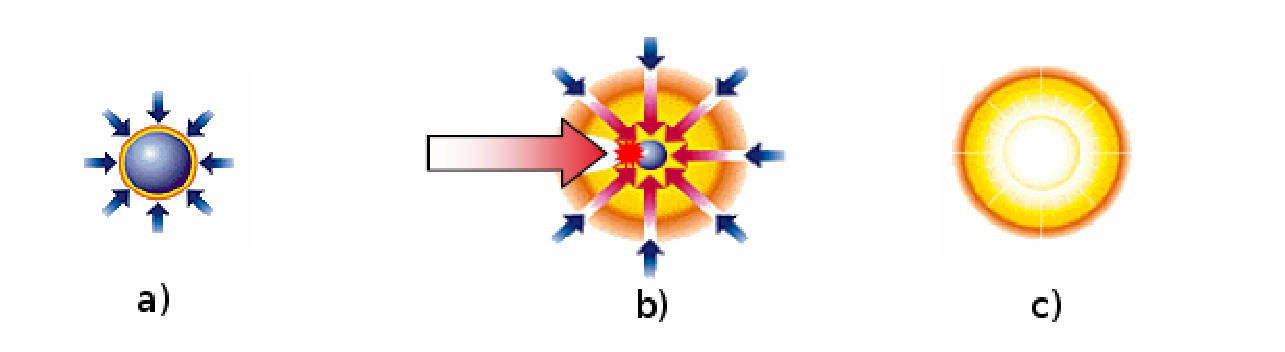
\includegraphics[width=0.8\textwidth]{images/FastStages}
	\caption{Les pas dans le processus de l'allumage ra\-pide : a) la compression, b) l'allumage et c) la combustion du combustible. Source: HiPER Technical background and conceptual design report \cite{hiper}, p. 13}
	\label{fig:FastStages}
\end{figure}

Ce projet sera financé par l'Union Européenne, le budget initial de recherche proposé est de 600 millions d'euros. Selon les informations du projet, la construction pourrait commencer en 2015 pour être mis en service 2020 \cite{hiper}.

\subsection{La fusion par confinement magnétique}
\begin{figure}[htb]
	\centering 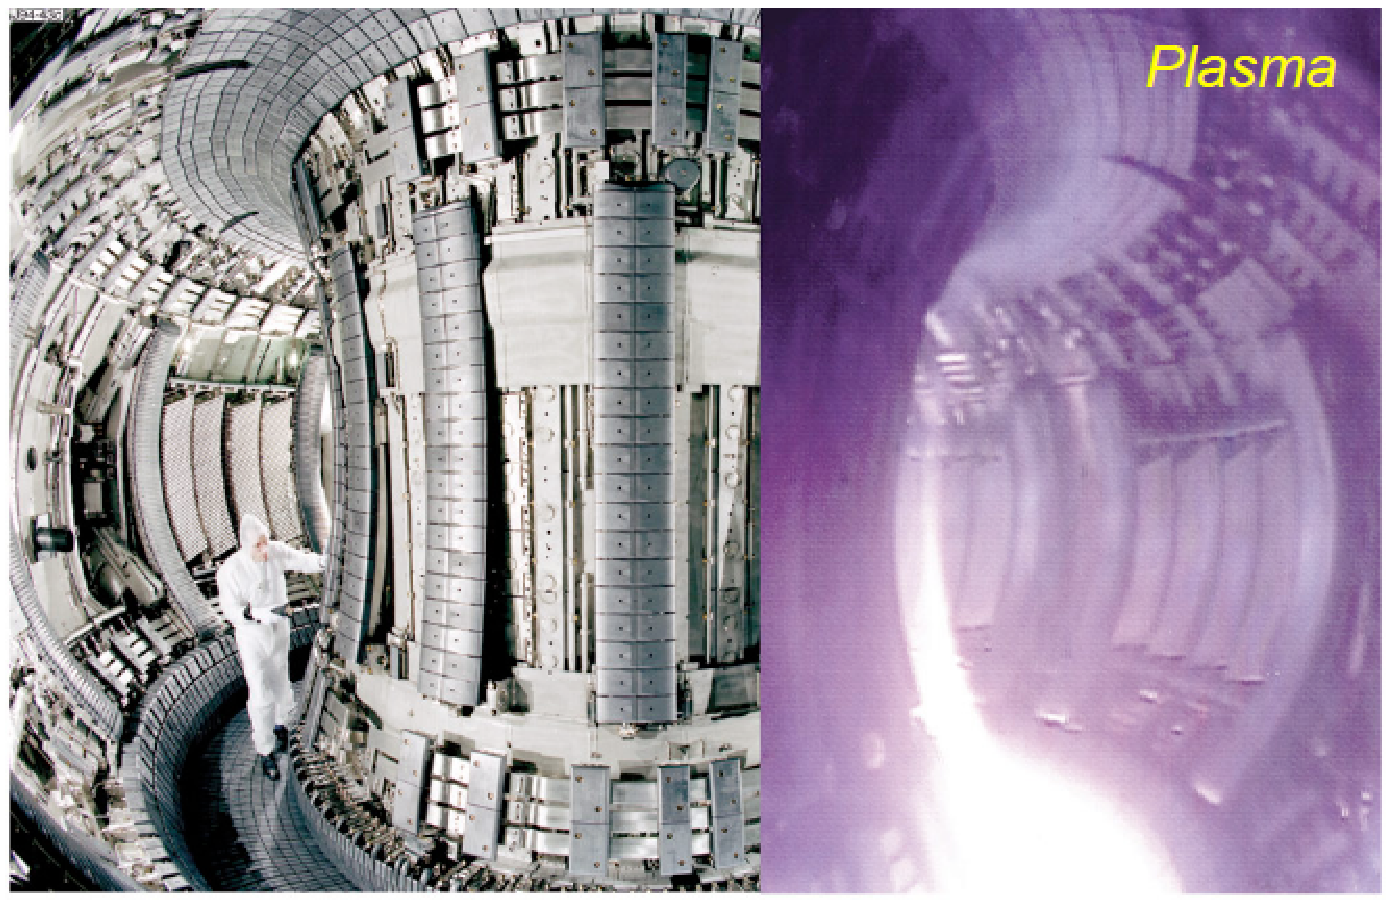
\includegraphics[width=0.6\textwidth]{images/jet}
	\caption{L'intérieur de <<JET>>, un réacteur de fusion par confinement magnétique en Angleterre. Source: \cite{iterheini}}
\end{figure}
La fusion par confinement magnétique fonctionne à base des champs magnétiques qui confinent et chauffent les combustibles. Il y a des configurations différentes comme les <<Tokamaks>>, les <<Stellerators>> et les <<Sphéromaks>> qui sont trop compliques pour les expliquer dans le cadre de ce travail. Malgré les configurations se distinguent par la manière de confiner et chauffer les particules, ils ont en commun que les réactions nucléaires ne prend pas place de façon répétitive mais continue. Dans la pratique, l'opération continue est encore un rêve car on n'a réalisé que des réactions qui ont duré des secondes\footnote{David Campbell: <<Inside ITER: Fusion, the Basics>> - Cadarache, 12 may 2009, p. 32 \cite{iterheini}}. Pour le réacteur <<ITER>> (<<International Thermonuclear Experimental Reactor>>), l'expérience plus grande de confinement magnétique, on prévoit une durée des réactions de 10 minutes au maximum. Le fait qu'ITER n'est qu'un pas dans le chemin à l'approvisionnement en énergie à base de fusion nucléaire se reflète aussi dans son nom qui signifie <<le chemin>> en latin.

Pour finir la partie du travail sur le confinement magnétique, quelques donnés sur ITER sont présentés: ITER a été proposé par Mikhaïl Gorbatchev lors du Sommet de Genève en novembre 1985 est l'effort plus international dans la recherche de fusion contrôlée. En décembre 2007, après une discussion longe sur le lieu du réacteur expérimental, on a commencé à construire ITER à Cadarache dans le sud de la France. Le budget du projet s'élève à 10 milliards d'euros. Actuellement, les pays membres du projet sont la Russie,
la Chine,
la Corée du Sud,
les États-Unis,
le Japon,
l'Union européenne et
l'Inde.

\section{Les aspects sociaux et écologiques}
\subsection{L'approvisionnement en deutérium et tritium} \label{dt}
Un des avantages plus grands de l'énergie à base de fusion nucléaire est le fait que les carburants sont disponibles en quantité énorme, au moins en théorie. En fait, un kilomètre cube de l'eau de la mer contient une quantité de deutérium qui est énergétiquement équivalente à toutes les réserves de pétrole\footnote{HiPER Technical background and conceptual design report \cite{hiper}, p. 12}. Le problème plus dure à solutionner est l'approvisionnement en tritium. Comme le tritium n'est pas un élément stable et a une demi-vie de 12 ans, il n'y a qu'env. 3,5 kg de production naturelle dans la terre\footnote{D. Lal und B. Peters: <<Cosmic ray produced radioactivity on the earth>>. Handbuch der Physik, vol. 46/2, p. 551–612, Springer, Berlin, 1967}. Au même temps, un réacteur futur d'une puissance éléctrique 1 GW aurait besion de env. 100 - 200 kg de tritium par an. Il faut donc le produire à base d'une réaction nucléaire:
\begin{equation}
^6 \text{Li} + n \rightarrow ^4 \text{He} + ^3 \text{T}
\end{equation}
Ça veut dire qu'il faut le produire à base du lithium, un élément qui est disponible en quantité suffisante. Le hic est que la production de tritium à cette manière serait seulement économiquement rentable si on pourrait le produire à base des neutrons de la réaction de fusion (eq. \ref{eqn:DTfusion}) même\footnote{M. E. Sawan, M. Abdou: <<Physics and technology conditions for attaining tritium self-sufficiency for the DT fuel cycle>>, Fusion Engineering and Design, éd. 81, 2006, p. 1143 \cite{tritiumself}}. C'est un des buts d'ITER et des autres expériences grandes de vérifier cette technologie. Il faut remarquer qu'il y a des opinions critiques par rapport à la réalisation de ce processus\footnote{Michael Dittmar: <<The Nuclear Energy Option facts and fantasies>>, ASPO06 Conference Cork, 17-18 septembre 2007, p. 20 \cite{dittmar}}.

Malgré cela, la production mondiale de lithium en 2008 s'élève à 27 400 ton\-nes\footnote{U.S. Geological Survey: <<Lithium Statistics and Information>>, 2009 \cite{usgs}}, beaucoup plus que les réacteurs de fusion en auront besoin dans le futur proche. Une conséquence des carburants utilisés est donc qu'il n'y aura pas de problème de transport ni de pénurie. Comme ni le deutérium ni le lithium sont des éléments radioactifs, ni l'exploitation ni le transport serait un péril pour la santé, au moins par rapport à l'exposition aux rayonnements.

\subsection{Le risque d'un accident}
Un avantage par rapport à la technologie de fission nucléaire est que le risque d'une réaction en chaine incontrôlée n'existe pas. D'abord, la réaction de fusion doit être entretenue avec des dépenses grandes (un champ magnétique, un laser de haute puissance, etc.) et une interruption de ces mécanismes de confinement résulte en une interruption de la réaction en conséquence. Deuxièmement et contrairement aux réacteurs de fission, les quantités de carburant dans le cœur du réacteur seraient petites et arrêter le ravitaillement en carburant suffirait pour arrêter la réaction. Le péril plus grand d'une émission de matériel radioactif viendrait d'un défaut du refroidissement du confinement de lithium. Même dans ce cas, des calculations ont démontré que la chaleur restée ne pourrait pas fondre les barrières du confinement. Dans le pire des cas, par exemple le crash d'une avion sur le site du réacteur, tout l'inventorie de tritium (env. 1 kg) pourrait être libéré. En assumant les pires conditions de temps, seulement le périmètre du site devrait être évacué\footnote{T. Hamacher et A.M. Bradshaw: <<Fusion as a future power source: Recent achievements and prospects>>, World Energy Council 18ème Congres, Buenos Aires, octobre 2001, p. 12 \cite{hamacher}}.

\subsection{Le problème des déchets radioactifs}
%
%
% Hier sollte ich mir mal auf deutsch auflisten, was ich schreiben will:
% - Unterschied zur Kernspaltung: es tritt als Abfallquelle eigentlich nur Punkt 2 auf
% - daher kein hochradioaktiver Abfall (Paper für Vergleich zitieren)
% - Physikalische Gründe für rad. Abfall: a) nicht verbrauchter Brennstoff, b) Neutroneneinfang, c) Produkte der Reaktion selbst (Spaltprodukte)
%
%Enthaltene Radionuklide
%
%An Radionukliden kommen in radioaktiven Abfällen aus Kernkraftwerken die folgenden wesentlichen Stoffgruppen vor:
%
%   1 * Spaltprodukte, also die bei der Kernspaltung entstehenden „Bruchstücke“. Diese sind zum größten Teil sehr kurzlebig (z. B. Iod-131, etc.), jedoch sind auch einige längerlebig (z. B. Cäsium-137, Strontium-90 etc.) oder langlebig (z. B. Iod-129 etc.).
%   2 * Aktivierungsprodukte. Dies sind ursprünglich nichtradioaktive Materialien aus dem Reaktor oder dessen Umgebung, die durch Neutroneneinfang von Spalt-Neutronen in radioaktive Nuklide umgewandelt wurden (prominentestes Nuklid ist hier Cobalt-60).
%   3 * Erbrüteter Kernbrennstoff, z. B. Plutonium-239, das durch Neutroneneinfang und zwei anschließende Betazerfälle aus Uran-238 gebildet wird, sowie das aus Plutonium-239 durch zwei Neutroneneinfänge erbrütete Plutonium-241.
%   4 * Erbrütete weitere Transurane, z. B. Americium-241, das durch mehrfachen Neutroneneinfang aus Plutonium-239 über Plutonium-240 und -241 mit nachfolgendem Betazerfall entsteht.
%   5 * Unverbrauchter ursprünglicher Brennstoff (Uran-235, Plutonium-239 und -241)
%   6 * Nicht in Plutonium umgewandeltes Uran-238
%
%
%
% Gute Übersicht: http://fusedweb.llnl.gov/faq/section2-energy/part2-enviro.txt (auf platte unter othershit)
%
%

Contrairement à la fission, la fusion nucléaire même (eq. \ref{eqn:DTfusion}) ne produit pas d'éléments radioactifs parce que l'hélium est un élément stable. Le problème est plutôt que le neutron rapide qui est produit par la fusion peut être capté par des éléments stables qui deviennent en conséquence instables. Ce processus nucléaire a lieu dans le système de confinement autour du réacteur. C'est un objet de recherche de construire un réacteur qui utilise des matériels appropriés pour que les demi-vies des éléments résultants soient les plus courtes possibles.

Un étude japonais\footnote{Y. Seki et al.: <<Preliminary Comparison of Radioactive Waste Disposal Cost
for Fusion and Fission Reactors>>, Journal of Fusion Energy, éd. 16, numéro 3, 1997, \cite{seki}} s'est occupé pour comparer les coûts du traitement et les quantités des déchets à celles d'un réacteur à fission: 

\begin{itemize}
\item Le traitement des déchets, dépendant du système de confinement du réacteur, coûterait entre 18 \% et 95 \% par rapport à un réacteur à fission, si les coûts du stockage intermédiaire sont inclus.
\item Les quantités de déchets générées pendant l'opération et après le decommissionnement d'un réacteur à fission de l'age de 30 ans et un réacteur à fusion de l'age de 20 ans sont presqu'équivalentes pour les faibles et moyennes activités.
\item Un réacteur à fusion produirait pas de déchets d'activité forte qui devraient être stockés géologiquement au moins 600 mètres sous terre.
\end{itemize}

Un réacteur à base de la réaction entre deutérium et tritium est donc loin de ne pas produire des déchets nucléaires. Pour le projet ITER, on estime qu'env. 30,000 tonnes de déchets radioactives resteraient après le decommissionnement du réacteur, qui résulteraient en env. 6000 tonnes de matériel radioactive après 100 ans\footnote{ITER: <<Summary of the
ITER
Final Design Report>>, juillet 2001, p. 57, \cite{itersafety}}. Seulement d'autres réactions de fusion qui n'emmétraient pas de neutrons énergétiques au prix d'être encore plus difficile à réaliser offriraient une source d'énergie entièrement libre de déchets nucléaires. 

%On prévoit que les déchets d'un réacteur désactivé seraient radiotoxiquement équivalents a celles d'une centrale à charbon pendant 500 ans\footnote{T. Hamacher et A.M. Bradshaw: <<Fusion as a future power source: Recent achievements and prospects>>, World Energy Council 18ème Congres, Buenos Aires, octobre 2001, p. 13 \cite{hamacher}}. 
\subsection{Le problème de la prolifération d'armes nucléaires}
Comme la fusion est une technologie nucléaire, la question sur la prolifération militaire apparait immédiatement. Les grandes expériences comme ITER en France ou NIF aux États-Unies vont également amener à une grande croissance du savoir-faire nucléaire et à des facilités pour l'appliquer. Un étude, crée par André Gsponer et Jean-Pierre Hurni, deux physiciens et opposants de l'énergie nucléaire, s'est occupé de ce problème\footnote{A. Gsponer, J.-P.
Hurni: <<ITER and the Nuclear Weapons Proliferation Implications
of Thermonuclear Fusion
Energy Systems>>, \url{http://arxiv.org/abs/physics/0401110}, 2004, p.38,\cite{gsponer}}. En suivante, je vais brièvement le présenter et en tirer quelques conséquences.

\subsubsection{L'abondance en neutrons}
Pendant que la fission produit entre deux et trois (2,5 en moyenne) neutrons et env. 200 MeV d'énergie par noyau fissionné, la fusion ne produit que 17,6 MeV d'énergie et un neutron par noyau fusionné. Pour générer la même quantité d'énergie d'une réaction à fission, on a besoin de $200 / 17,6$ MeV $\approx 10$ réactions de fusion, en émettant 10 neutrons au lieu de 2,5 en conséquence. C'est pour ça que la fusion est parfois appelée <<riche en neutrons, pauvre en énergie>> par rapport à la fission nucléaire. Cette richesse de neutrons signifie une efficacité de production de plutonium et tritium bien élevée, deux matériaux dont le militaire a besoin pour produire des armes nucléaires. Selon l'étude de Gsponer et Hurni, une facilité dédiée à la production militaire était plus facile à cacher: Par rapport à la quantité produite, la production de chaleur, de déchets nucléaires et de noyaux traçables était au moins dix fois plus petite.

\subsubsection{L'abondance en tritium}
Indépendant du type de réacteur, la quantité de tritium dont on aurait besoin s'élèverait à env. 0,5 kg par jour (entre 100 kg et 200 kg par an), dans une centrale d'une puissance électrique de 1 GW. Comme déjà expliqué, le tritium est un élément instable et devrait être généré par le réacteur même en conséquence. Dans les Etats-Unies, la quantité de tritium stockée pour des raisons militaires s'élève à env. 100 kg. Comme la demi-vie de tritium est env. 12,3 ans, la moité de 100 kg doit être produite pendant cette période de temps pour entretenir cette masse. La quantité annuelle dont le militaire a besoin est donc $50$ kg $/ 12,3$ ans $\approx 4$ kg par an qui pourrait facilement être produit dans une centrale à fusion.

Il y a deux autres aspects à considérer concernant la prolifération en tritium:

\begin{itemize}
\item Pour <<améliorer>> la puissance des armes nucléaires à fission à grande efficacité, une quantité tant petite comme 2 g suffit. 
\item Les arsenals nucléaires futures vont probablement être basé sur les armes à <<fusion pure>>. Ces armes de quatrième génération auront besoin de quantités petites de tritium. Pour une efficacité relativement pauvre de 20~\%, chaque milligramme de tritium serait équivalente à env. 100 kg de TNT. %Si une centrale à fusion pourrait approvisionner en 0,05 kg de tritium par jour, cette quantité serait suffisante pour produire 5000 des ogives explosives par jour, chaque étant équivalente à une tonne de TNT.
\end{itemize}
Considérant les difficultés qui déjà existent avec le contrôle du plutonium, un tel niveau de contrôle de tritium apparaît pratiquement impossible.

\section{Conclusion} %TODO: Titel sollte beinhalten dass auch ein ausblick im bezug auf die nachhaltige entwicklung gegeben wird
Pour répondre à la question du titre de ce travail, je suis arrivé aux conclusions suivantes:
\begin{itemize}
\item L'abondance des carburants nécessaires pour la fusion dans la terre, pour vu que la génération de tritium dans le réacteur soit atteint, est l'avantage plus grand de la fusion.
\item Comme les centrales à fusion produiraient une quantité de déchets radioactifs considérable, on ne peut pas parler d'une source d'énergie propre. Malgré cela, les bénéfices par rapport aux énergies fossiles sont l'absence de gaz à effet de serre, par rapport à la fission nucléaire l'absence de déchets d'une demi-vie longue qui devraient être stockés géologiquement.
\item Même si le problème des réactions en chaîne incontrôlées n'existe pas, un péril grave dans la technologie de la fission nucléaire, la fusion nucléaire ne peut pas être appelée sécuritaire à cause des problèmes de prolifération militaire durement solubles.
\end{itemize}
% TODO: Ueberleiten und sagen dass nun ein etwas subjektiverer und weniger wissenschaftlicher teil kommt.
Au total, je ne dirais pas que la fusion nucléaire est la solution parfaite qui pourrait alimenter le monde en énergie. Même si les centrales à fusion seraient dis\-po\-ni\-bles immédiatement, quelque chose qui est loin d'être la réalité pour le moment, on ne pourrait pas les considérer pour éviter des émissions de gaz à effet de serre à cause des inconvénients présentés.
%TODO: Weg mit der philosophischen Kacke, sagen dass es schwer war die Informationen zusammenzutragen und einen Ueberblick zu bekommen

%
%Pendent les recherches pour ce travail, je suis devenu assez désillusionné et je suis arrivé à quelques conclusions plus générales que je voudrais aussi présenter à ce lieu, même si elles pourraient apparaître très subjectives: En considérant les capacités des énergies renouvelables que je préfère aux centrales à fusion, je suis arrivé à l'opinion qu'une source d'énergie qui ne libère pas de gaz à effet de serre et génère les grandes quantités d'énergie dont on a besoin n'existe pas.
%Il faudrait plutôt réduire la consommation d'énergie à grande échelle. Je crois qu'une telle réduction ne serait possible qu'en cas d'un changement de notre mode de vie. À mon avis, il faut finalement accepter qu'un mode de vie durable consiste en s'abstenir de certaines choses qui apparaissent normales au monde occidental du présent, par exemple:
%\begin{itemize}
%\item Le confort de mobilité presqu'illimité, indépendant si les voitures et avions futurs consommeront des carburants fossiles ou d'électricité.
%\item Wat noch...? Teure und aufwendige Reisen?? 
%\item Le dogme de la croissance de production illimitée qui implique à créer continuellement des demandes nouvelles. C'est dure à imaginer un surplus en production sans une augmentation en consommation d'énergie et de ressources.
%\item etc.
%\end{itemize}
%TODO: gut begruenden, warum verzicht auf diese sachen notwendig ist.
% Philosophisch ausgedrueckt: es gibt probleme ohne Loesung

\begin{thebibliography}{99}
\bibitem{dem} W. Demtröder: Experimentalphysik 4 (Kern-, Teilchen- und Astrophysik), Springer-Verlag Berlin Heidelberg New-York, 2ème édition, 2004
% TODO: titel bei den naechsten beiden hier
\bibitem{iterMission} \url{http://www.iter.org/proj/Pages/ITERMission.aspx}
\bibitem{nif} \url{https://lasers.llnl.gov/programs/ife/how_ife_works.php}
\bibitem{iterheini} David Campbell: <<Inside ITER: Fusion, the Basics>> - Cadarache, 12 may 2009, \url{http://www-arch.iter.org/newsline/issues/73/FusionBasics_DavidCampbell.pdf}
\bibitem{hiper} <<HiPER Technical background and conceptual design report 2007>>, \url{http://www.hiper-laser.org/docs/tdr/HiPERTDR2.pdf}
\bibitem{fusionwiki} \url{http://fr.wikipedia.org/wiki/Fusion_nucleaire}
\bibitem{tritiumself} M. E. Sawan, M. Abdou: <<Physics and technology conditions for attaining tritium self-sufficiency for the DT fuel cycle>>, Fusion Engineering and Design, éd. 81, 2006, p. 1131–1144, \url{http://www.fusion.ucla.edu/abdou/abdou\%20publications/2006/FED-v81-SawanPhysics.pdf}
\bibitem{dittmar} Michael Dittmar: <<The Nuclear Energy Option facts and fantasies>>, ASPO06 Conference Cork, 17-18 septembre 2007, \url{http://www.aspo-ireland.org/contentfiles/ASPO6/3-2_APSO6_MDittmar.pdf}
\bibitem{usgs} U.S. Geological Survey: <<Lithium Statistics and Information>>, 2009, \url{http://minerals.usgs.gov/minerals/pubs/commodity/lithium/mcs-2009-lithi.pdf}
\bibitem{hamacher} T. Hamacher et A.M. Bradshaw: <<Fusion as a future power source: Recent achievements and prospects>>, World Energy Council 18ème Congres, Buenos Aires, octobre 2001, \url{http://web.archive.org/web/20040506065141/http://www.worldenergy.org/wec-geis/publications/default/tech_papers/18th_Congress/downloads/ds/ds6/ds6_5.pdf}
\bibitem{seki} Y. Seki et al.: <<Preliminary Comparison of Radioactive Waste Disposal Cost
for Fusion and Fission Reactors>>, Journal of Fusion Energy, éd. 16, numéro 3, 1997
\bibitem{gsponer} A. Gsponer, J.-P.
Hurni: <<ITER and the Nuclear Weapons Proliferation Implications
of Thermonuclear Fusion
Energy Systems>>, 2004, \url{http://arxiv.org/abs/physics/0401110}
\bibitem{itersafety} ITER: <<Summary of the
ITER
Final Design Report>>, juillet 2001, \url{http://fire.pppl.gov/iter_summary_FDR2001.pdf}

\end{thebibliography}

\section*{Vocabulaire}
\begin{tabular}{|l|l|} %TODO: alphabetisch sortieren
\hline
noyau (m.) & (Atom-)kern \\
fission nucléaire (f.) & Kernspaltung \\
fusion nucléaire (f.) & Kernfusion \\
défaut de masse (m.) & Massendefekt \\
gain (m.) & Gewinn \\
étincelle d'allumage (f.) & Zündfunke \\
charge électrique (f.) & Elektrische Ladung \\
particule (f.) & Teilchen \\
intertie (f.) & Trägheit \\
faisceau (m.) & (Strahlen-) Bündel \\
rayon (f.) & Strahl \\
fusion par confinement magnétique (f.) & Fusion mittels magn. Einschlusses \\
fusion par confinement inertiel (f.) & Trägheitsfusion\\
combustible (m.) & Brennstoff \\
réaction auto-entretenue (f.) & Selbsterhaltende Reaktion \\
réaction en chaîne (f.) & Kettenreaktion \\
approvisionnement en énergie (m.) & Energieversorgung \\
demi-vie (f.) & Halbwertszeit\\
ogive explosive (f.) & Sprengkopf, Gefechtskopf \\
\hline
\end{tabular}

\end{document}
